\documentclass[a4paper,14pt]{article}

\usepackage{comment} % Para comentar várias linhas ao mesmo tempo

%matemática
\usepackage{amsmath}
\usepackage{amssymb}

%diagramação
\usepackage{extsizes}
\everymath{\displaystyle}
\usepackage{geometry}
\usepackage{fancyhdr}
\usepackage{multicol}
\usepackage{graphicx}
\usepackage[brazil]{babel}
\usepackage[shortlabels]{enumitem}
\usepackage{cancel}
\usepackage{textcomp}
\usepackage{tcolorbox}

%tabelas
\usepackage{array} % Para melhor formatação de tabelas
\usepackage{longtable}
\usepackage{booktabs}  % Para linhas horizontais mais bonitas
\usepackage{float}   % Para usar o modificador [H]
\usepackage{caption} % Para usar legendas em tabelas
\usepackage{wrapfig} % Para usar tabelas e figuras flutuantes
\usepackage{xcolor} % Para cores do fundo de tabelas
\usepackage{colortbl} % Para cores do fundo de tabelas

%tikzpicture
\begin{comment}
	\usepackage{tikz}
	\usepackage{scalerel}
	\usepackage{pict2e}
	\usepackage{tkz-euclide}
	\usetikzlibrary{calc}
	\usetikzlibrary{patterns,arrows.meta}
	\usetikzlibrary{shadows}
	\usetikzlibrary{external}
\end{comment}


%pgfplots
\usepackage{pgfplots}
\pgfplotsset{compat=newest}
\usepgfplotslibrary{statistics}
\usepgfplotslibrary{fillbetween}

%colours
\usepackage{xcolor}



\columnsep=2cm
\hoffset=0cm
\textwidth=8cm
\setlength{\columnseprule}{.1pt}
\setlength{\columnsep}{2cm}
\renewcommand{\headrulewidth}{0pt}
\geometry{top=1in, bottom=1in, left=0.7in, right=0.5in}

\pagestyle{fancy}
\fancyhf{}
\fancyfoot[C]{\thepage}

\begin{document}
	
	\noindent\textbf{6FMA126 - Matemática} 
	
	\begin{center}Revisão: equações e módulo (Versão estudante)
	\end{center}
	
	\noindent\textbf{Nome:} \underline{\hspace{10cm}}
	\noindent\textbf{Data:} \underline{\hspace{4cm}}
	
	%\section*{Questões de Matemática}
	
	\begin{multicols}{2}
	    \noindent Lembre-se: \\ \textbf{1.} Para resolver equações, devemos: \\
	    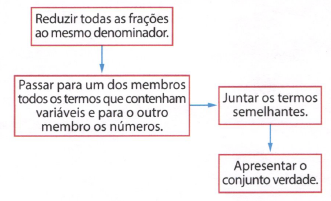
\includegraphics[width=1\linewidth]{6FMA126_imagens/imagem1} \\\\
	    \textbf{2.} O módulo ou valor absoluto de um número inteiro é a distância desse número até o zero na reta orientada.
		\noindent\textsubscript{--------------------------------------------------------------------------}
		\begin{enumerate} 
			\item Resolver as equações no universo $U = \mathbb{Q}$
			\begin{enumerate}[a)]
				\item $3x - 7 = 0$ \\\\\\\\\\\\\\\\\\\\
				\item $0x - 8 = 0$ \\\\\\\\
				\item $0x + 0 = 0$ \\\\\\\\\\\\\\\\\\\\
				\item $2 - x = 9$ \\\\\\\\\\\\\\\\\\\\
				\item $5a - 3 = -a + 11$ \\\\\\\\\\\\\\\\\\\\\\
			\end{enumerate}
			\item Represente os números a seguir na reta:
			\begin{enumerate}[a)]
				\item $|-5|$ \\
				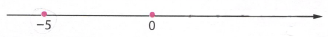
\includegraphics[width=1\linewidth]{6FMA126_imagens/imagem2} \\\\
				\item $|4|$ \\
				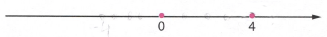
\includegraphics[width=1\linewidth]{6FMA126_imagens/imagem3} \\\\
				\item $-|-3|$ \\
				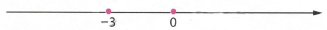
\includegraphics[width=1\linewidth]{6FMA126_imagens/imagem4} \\\\
				\item $-|6|$ \\
				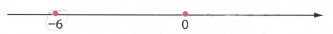
\includegraphics[width=1\linewidth]{6FMA126_imagens/imagem5} \\\\
			\end{enumerate}
			\item Dado $x \in \mathbb{Z}$, defina $|x|$, isto é, diga quanto vale $|x|$. \\\\\\\\\\\\\\\\\\\\\\\\\\\\\\\\\\
			\item Calcular:
			\begin{enumerate}[a)]
				\item $|-6|$ \\\\\\
				\item $|21 - 8|$ \\\\\\
				\item $|12 - 15|$ \\\\\\
				\item $|5 - 6 + 7 - 8|$ \\\\\\
				\item $|-|-6||$ \\\\\\
				\item $-|-6|$ \\\\\\
			\end{enumerate}	
			%1 e 2
			\item Resolver as equações ($U = \mathbb{Q}$).
			\begin{enumerate}[a)]
				\item $2x - 16 = 0$ \\\\\\\\\\\\
				\item $3y + 18 = 0$ \\\\
				\item $4x + 12 = 3x + 15$ \\\\\\\\\\\\\\
				\item $\frac{a}{2} - \frac{a}{5} - a - 14$ \\\\\\\\\\\\
				\item $\frac{2x + 1}{3} = \frac{2}{7} + \frac{5x}{6}$ \\\\\\\\\\\\
			\end{enumerate}	
			\item Calcular:
			\begin{enumerate}[a)]
				\item $||-7||$ \\\\\\
				\item $||1 - 3| - 12|$ \\\\\\
				\item $|7 - |1 - 3| + 2|$ \\\\\\
			\end{enumerate}	
		\end{enumerate}
		$~$ \\ $~$ \\ $~$ \\ $~$ \\ $~$ \\ $~$ \\ $~$ \\ $~$ \\ $~$ \\ $~$ \\ $~$ \\ $~$ \\ $~$ \\ $~$ \\ $~$ \\ $~$ \\ $~$ \\ $~$ \\ $~$ \\ $~$ \\ $~$ \\ $~$ \\ $~$ \\ $~$ \\ $~$ \\ $~$ \\ $~$ \\ $~$ \\ $~$ \\ $~$ \\ $~$ \\ $~$ \\ $~$ \\ $~$ \\ $~$ \\ $~$ \\ $~$ \\ $~$ \\ $~$ \\ $~$ \\ $~$ \\ $~$ \\ $~$ \\ $~$ \\ $~$ \\ $~$
	\end{multicols}
\end{document}